%%%%%%%%%%%%%%%%%%%%%%%%%%%%%%%%%%%%%%%%%
% Arsclassica Article
% LaTeX Template
% Version 1.1 (1/8/17)
%
% This template has been downloaded from:
% http://www.LaTeXTemplates.com
%
% Original author:
% Lorenzo Pantieri (http://www.lorenzopantieri.net) with extensive modifications by:
% Vel (vel@latextemplates.com)
%
% License:
% CC BY-NC-SA 3.0 (http://creativecommons.org/licenses/by-nc-sa/3.0/)
%
%%%%%%%%%%%%%%%%%%%%%%%%%%%%%%%%%%%%%%%%%

%----------------------------------------------------------------------------------------
%	PACKAGES AND OTHER DOCUMENT CONFIGURATIONS
%----------------------------------------------------------------------------------------

\documentclass[
12pt, % Main document font size
a4paper, % Paper type, use 'letterpaper' for US Letter paper
oneside, % One page layout (no page indentation)
%twoside, % Two page layout (page indentation for binding and different headers)
headinclude,footinclude, % Extra spacing for the header and footer
BCOR5mm, % Binding correction
]{scrartcl}
\usepackage[english]{babel}
\usepackage{url}
\usepackage{graphicx}
\usepackage{subcaption}
\usepackage{float}
\usepackage{titlepic}
\usepackage{epigraph}
\usepackage{mathcomp}
\usepackage{textcomp}
\usepackage[LGR,T1]{fontenc}
\usepackage{amsmath}
\usepackage{url}
\usepackage{sectsty}
\usepackage[dvipsnames,table,xcdraw,svgnames]{xcolor}
\usepackage{listings}
\usepackage{booktabs}
\newcommand{\textgreek}[1]{\begingroup\fontencoding{LGR}\selectfont#1\endgroup}
\usepackage{url}
\lstset{language=R,
    basicstyle=\small\ttfamily,
    stringstyle=\color{DarkGreen},
    otherkeywords={0,1,2,3,4,5,6,7,8,9},
    morekeywords={TRUE,FALSE},
    deletekeywords={data,frame,length,as,character},
    keywordstyle=\color{blue},
    commentstyle=\color{DarkGreen},
}


%%%%%%%%%%%%%%%%%%%%%%%%%%%%%%%%%%%%%%%%%
% Arsclassica Article
% Structure Specification File
%
% This file has been downloaded from:
% http://www.LaTeXTemplates.com
%
% Original author:
% Lorenzo Pantieri (http://www.lorenzopantieri.net) with extensive modifications by:
% Vel (vel@latextemplates.com)
%
% License:
% CC BY-NC-SA 3.0 (http://creativecommons.org/licenses/by-nc-sa/3.0/)
%
%%%%%%%%%%%%%%%%%%%%%%%%%%%%%%%%%%%%%%%%%

%----------------------------------------------------------------------------------------
%	REQUIRED PACKAGES
%----------------------------------------------------------------------------------------

\usepackage[
nochapters, % Turn off chapters since this is an article        
beramono, % Use the Bera Mono font for monospaced text (\texttt)
eulermath,% Use the Euler font for mathematics
pdfspacing, % Makes use of pdftex’ letter spacing capabilities via the microtype package
dottedtoc % Dotted lines leading to the page numbers in the table of contents
]{classicthesis} % The layout is based on the Classic Thesis style

\usepackage{arsclassica} % Modifies the Classic Thesis package

\usepackage[T1]{fontenc} % Use 8-bit encoding that has 256 glyphs

\usepackage[utf8]{inputenc} % Required for including letters with accents

\usepackage{graphicx} % Required for including images
\graphicspath{{Figures/}} % Set the default folder for images
 % Include the structure.tex file which specified the document structure and layout
\sloppy
\hyphenation{Fortran hy-phen-ation} % Specify custom hyphenation points in words with dashes where you would like hyphenation to occur, or alternatively, don't put any dashes in a word to stop hyphenation altogether

%----------------------------------------------------------------------------------------
%	TITLE AND AUTHOR(S)
%----------------------------------------------------------------------------------------

\begin{document}



\title{\normalfont{A bird's-eye view on the habitability of exoplanets via statistical learning techniques}} % The article title

\subtitle{Project for the exam: Machine learning, statistical learning, deep learning and artificial intelligence} % Uncomment to display a subtitle


\author{Marzio De Corato} % The article author(s) - author affiliations need to be specified in the AUTHOR AFFILIATIONS block

\date{\today} % An optional date to appear under the author(s)

%\titlepic{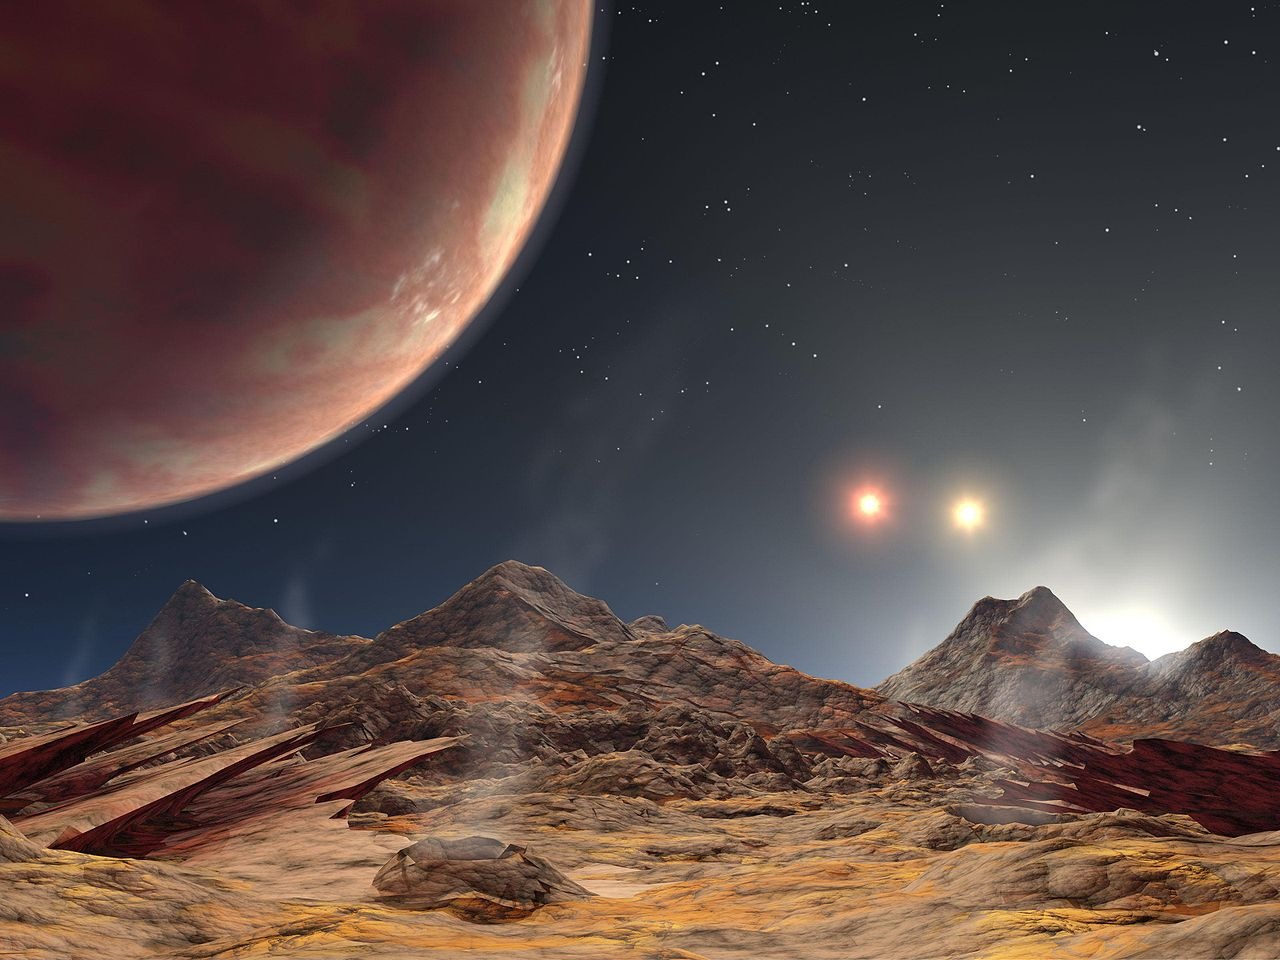
\includegraphics[width=\textwidth]{Pic/Triple-star_sunset.jpg}}


%----------------------------------------------------------------------------------------





%----------------------------------------------------------------------------------------
%	HEADERS
%----------------------------------------------------------------------------------------

\renewcommand{\sectionmark}[1]{\markright{\spacedlowsmallcaps{#1}}} % The header for all pages (oneside) or for even pages (twoside)
%\renewcommand{\subsectionmark}[1]{\markright{\thesubsection~#1}} % Uncomment when using the twoside option - this modifies the header on odd pages
\lehead{\mbox{\llap{\small\thepage\kern1em\color{halfgray} \vline}\color{halfgray}\hspace{0.5em}\rightmark\hfil}} % The header style

\pagestyle{scrheadings} % Enable the headers specified in this block

%----------------------------------------------------------------------------------------
%	TABLE OF CONTENTS & LISTS OF FIGURES AND TABLES
%----------------------------------------------------------------------------------------

\maketitle % Print the title/author/date block

\newpage
\setlength\epigraphwidth{.7\textwidth}
\epigraph{ "Listen to me again. Just outside the Galaxy are the Magellanic Clouds, where no human ship has ever penetrated. Beyond that are other small galaxies, and not very far away is the giant Andromeda Galaxy, larger than our own. Beyond that are galaxies by the billions. Our own Galaxy has developed only one species of an intelligence great enough to develop a technological society, but what do we know of the other galaxies? Ours may be atypical. In some of the others-perhaps even in all-there may be many competing intelligent species, struggling with each other, and each incomprehensible to us. Perhaps it is their mutual struggle that preoccupies them, but what if, in some galaxy, one species gains domination over the rest and then has time to consider the possibility of penetrating other galaxies" \newline (I.Asimov, Foundation and Earth)
}



\newpage


%----------------------------------------------------------------------------------------
%	ABSTRACT
%----------------------------------------------------------------------------------------

\section*{Abstract} % This section will not appear in the table of contents due to the star (\section*)
Among the different tools that are considered by scholars to challenge the physical science issues, the statistical learning techniques seems to provide a promising approach to challenge them \cite{carleo2019machine}. This approach can be used to tackle, one of the oldest problem of physical sciences:  the habitability of exoplanets and the possibility of the presence of life on them \cite{seager2013exoplanet}. This approach was previously used by scholars \cite{armstrong2020exoplanet}: here a group of statistical learning techniques (Decision Tree, Random Forest, Support-vector machines and Quadratic Discriminat analysis) were applied to a selected set of 500 planets. The performances of the different methods were also compared and using the confusion matrix and the ROC curve.

\nocite{*}
\setcounter{tocdepth}{2} % Set the depth of the table of contents to show sections and subsections only

\tableofcontents % Print the table of contents

%\listoffigures % Print the list of figures

%\listoftables % Print the list of tables


\newpage % Start the article content on the second page, remove this if you have a longer abstract that goes onto the second page

\section{Introduction}
The possibility of other form of life on other planets represented an issue that involved scientists as well as philosophers for different millennia of documented human history \cite{papagiannis1985historical}. During the XX century, due to the technological progress, such question moved from a pure speculative approach, as it was previously for Lucretius, Muhammad al-Baqir or Iordanus Brunus, to a more quantitative and scientific method. Furthermore it is interesting to point out that this research was undertaken when the exploration of the Earth was almost completed \cite{fleming2001barrow}. The exploration of space, and the investigation of other planets was largely boosted by the use of telescopes that measure the radiation also outside the visible spectrum and later with the space telescopes such as the NASA's Kepler. Finally the use of the space probes allowed a closer exploration of planets as wells of moons of solar system \cite{space_probes}. 
Only rocky planets are considered habitable \footnote{In principle also moons have to be considered, however for sake of simplicity here we take into account only planets}, so gaseous ones such as Jupiter or Saturn have to be considered not habitable (see Fig. \ref{exoplanet_populations} and \ref{PT_Confirmed}); second, as requested by all form of life in the Earth, an habitable planet requires that liquid water can be present \cite{seager2013exoplanet,mckay2014requirements,rothschild2001life} \footnote{Astrobiologist scholars also proposed that other form of life can come up without liquid water (see for instance \cite{rahm2016polymorphism}) however, for simplicity, here only planets that allows liquid water are considered habitable}. This feature is given, at first glance, by the radiation intensity $I$ that is bounded to the power radiation ($P$) produced by the star that host the planet and the respective distance $r$. Indeed by approximating a star as a point or a perfect sphere, a radiation with a spherical symmetry is produced; thus the integral that gives the power produced $P$: 
\begin{equation}
P=\int \textbf{I}\cdot \textit{d\textbf{A}}
\end{equation}
can be simplified as 
\begin{equation}
P=\lvert I \rvert \cdot A_{surf}=4\pi r^{2}
\end{equation}
and so  \footnote{Further details about this solution and the formalism by which it is obtained from the Maxwell equations can be found in Ref. \cite{feynman}.}
\begin{equation}
\lvert I \rvert=\dfrac{P}{4\pi r^{2}}
\end{equation}
Such relation establishes an interval for the distance $r$ where the stellar radiation is not too hot so that the water is the gas phase, and not to low so only the solid state phase is allowed. In the literature this interval is usually called habitable-zone \cite{kasting1993habitable}. However this represents a too simplified model since no atmospheric effect is taken in to account: indeed the surface temperature is also influenced by the greenhouse gases that allows to the host radiation to enter inside the planet but limits its escape \cite{seager2013exoplanet,forget2014possible}. Basically, as explained in figure \ref{Greenhouse-effect-t2} this is due to the fact that the greenhouse molecules, such as CO$_{2}$, vapour, CH$_{4}$, are excited by the infra-red radiation produced by the planet and remit it in all directions. As consequence the overall heat that is lost by the planet through infra-red radiation is reduced \cite{pierrehumbert2011infrared}, and so the surface temperature is increased. It is worth nothing that in principle the greenhouse effect does not reduce the habitability: on the contrary it allows to the planet to keep part of the heath received from the host star. On the other side, if the concentration of the greenhouse gases is too hight, and thus the the surface temperature abruptly increases, the planetary homoeostasis\cite{lovelock1974atmospheric,lovelock1982life,caldeira1992life} breaks and the water that is present on the planet escapes from it; this was probably the fate of Venus that lost his oceans \cite{way2016venus,luger2015extreme,seager2013exoplanet}. The conventional habitable zone can be extended if, for instance, we take in to account the fact that more massive planets are able to bound the H$_{2}$ (a greenhouse gas see Fig \ref{Planets_habitability_Seager}), thus also the mass of a planet is involved as factor for its habitability. Scholars \cite{tackley2012habitable} also focused on the tectonic phenomena that allows the recycling of atmospheric gases and produces a negative feedback for surface temperature \cite{walker1981negative}: this feature, at a first glance, is largely influenced by the presence of water \cite{korenaga2010likelihood,o2007geological} and weakly by the planet radius \cite{o2007geological} and mass \cite{korenaga2010likelihood}.
  

\begin{figure}[h]
\begin{center}
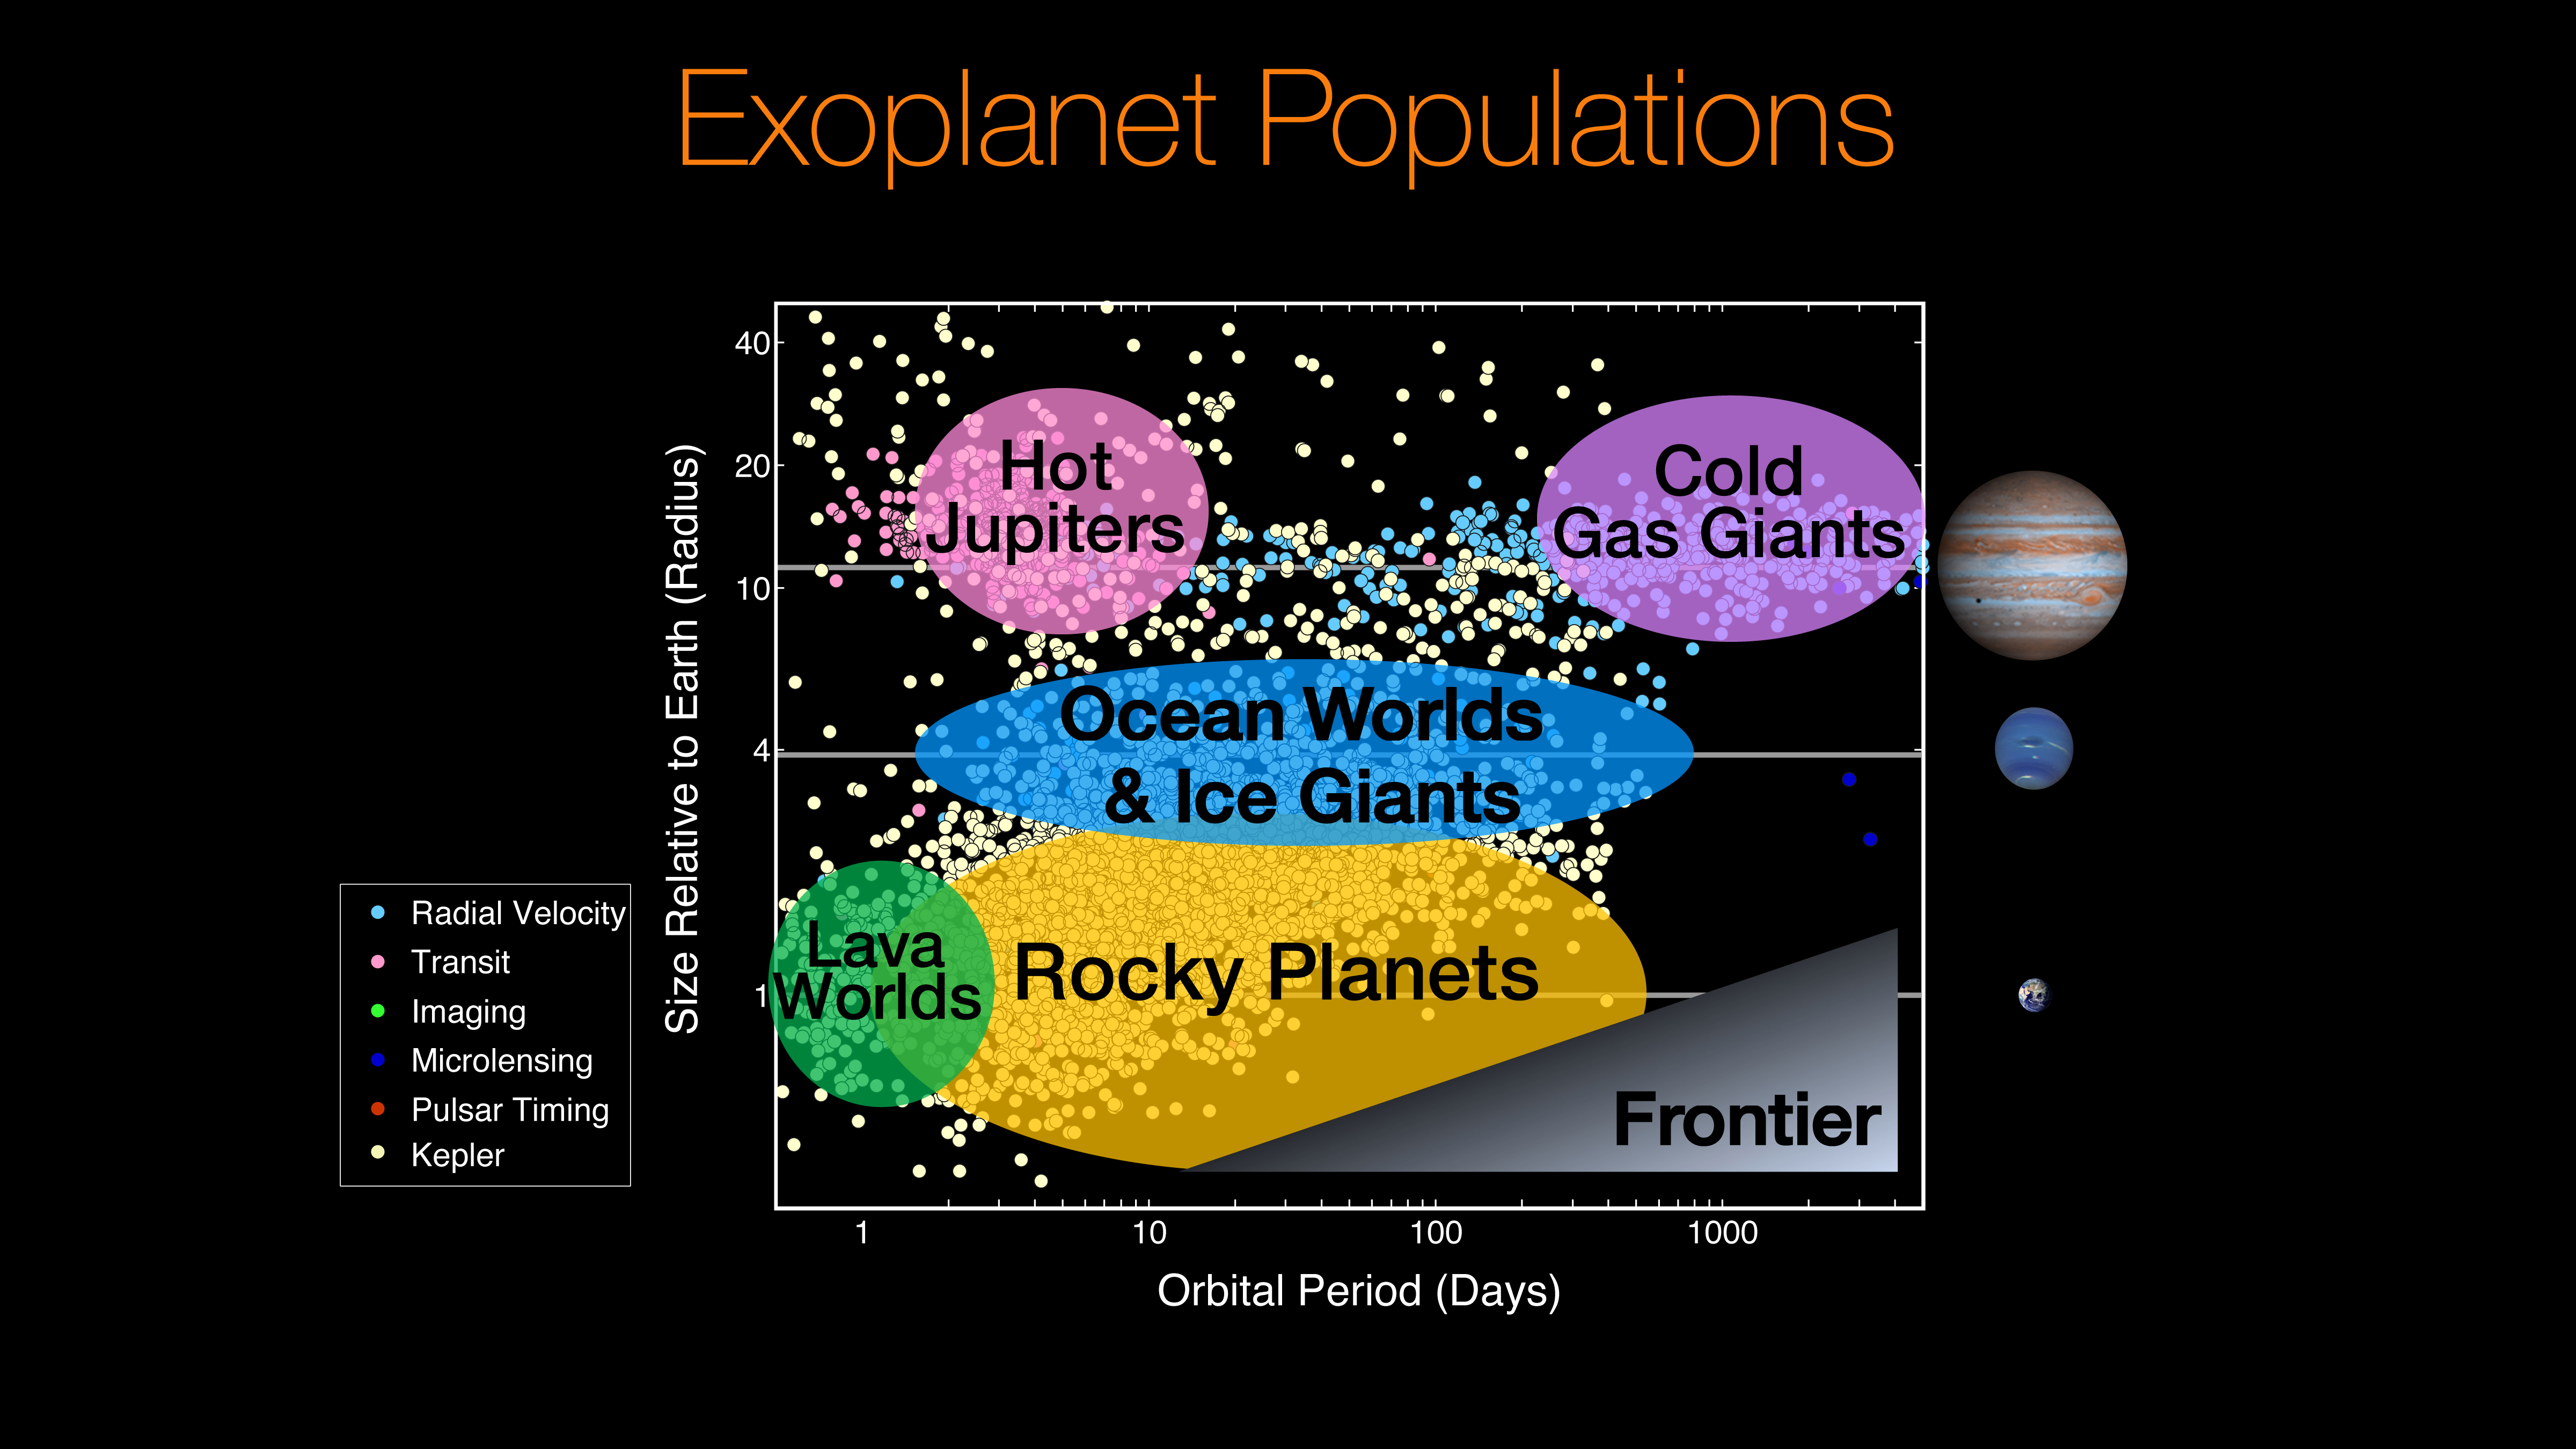
\includegraphics[width=1\textwidth]{Pic/press-web25_exoplanet_populations.jpg}
\caption{A NASA plot about the possible type of exoplanets given their orbital period and size. Image taken from \cite{exoplanet_populations}}
\label{exoplanet_populations}
\end{center}
\end{figure}

\begin{figure}[h]
\begin{center}
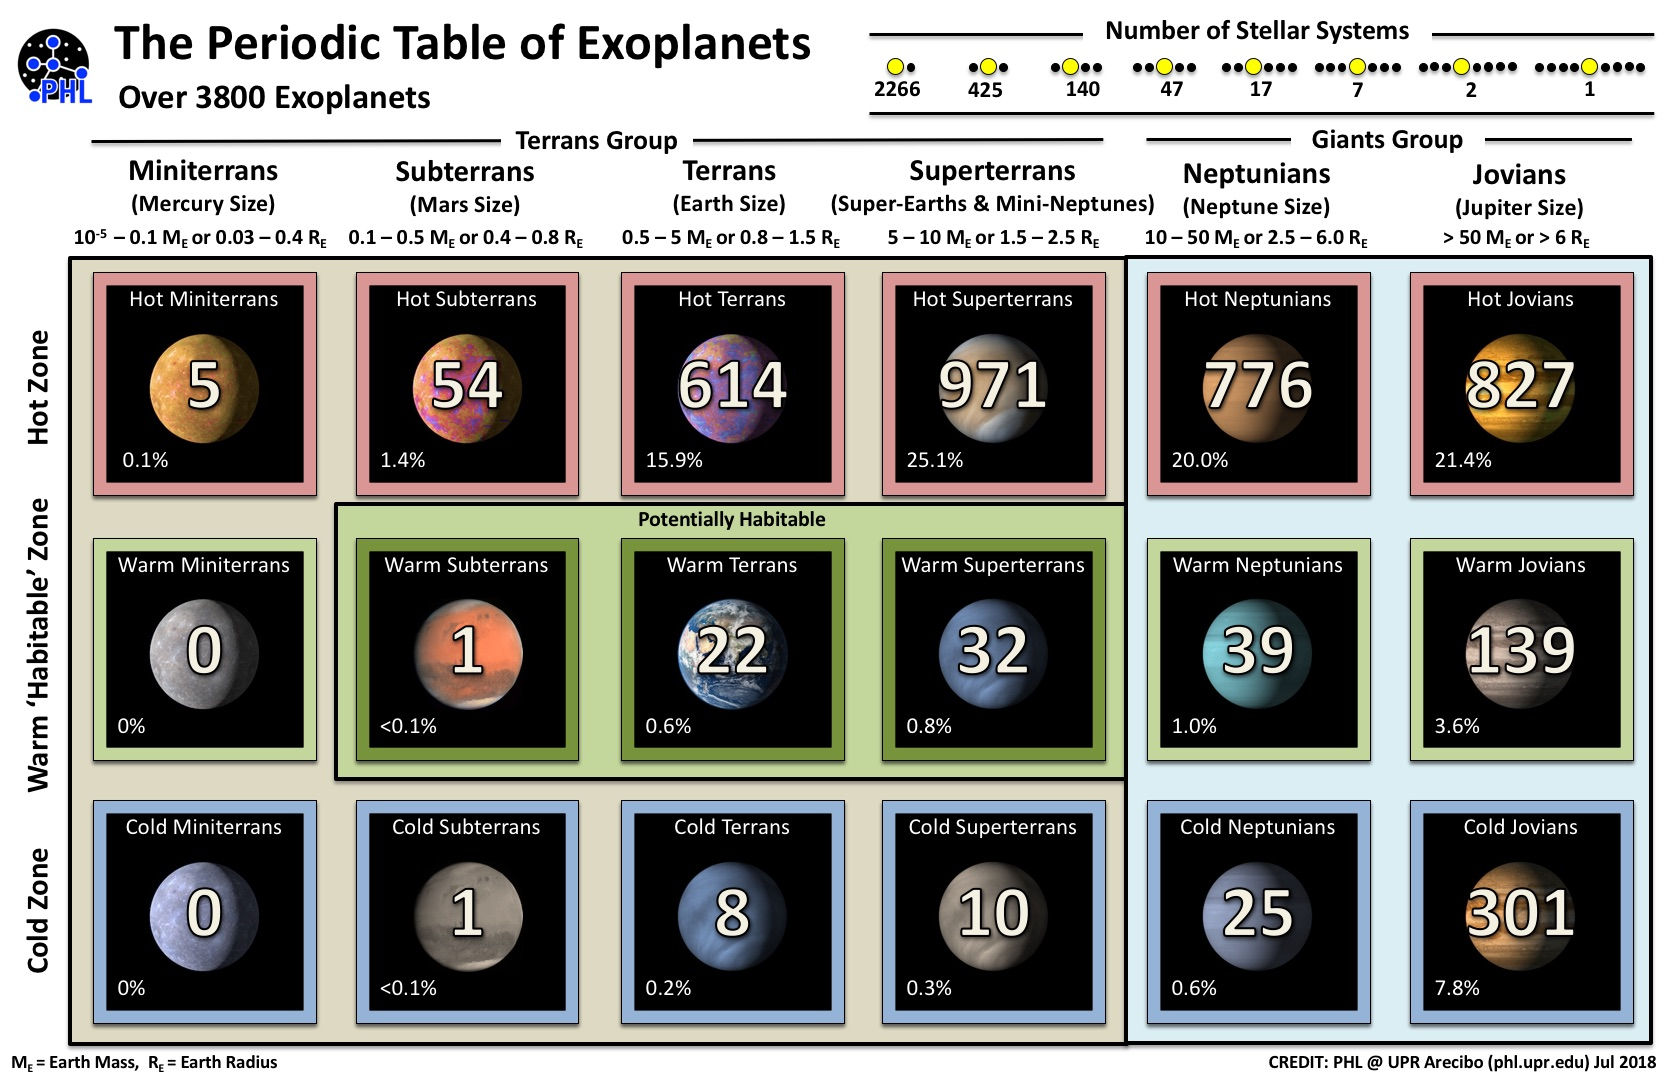
\includegraphics[width=1\textwidth]{Pic/PT_Confirmed.jpg}
\caption{PHL @ UPR Arecibo classification of the different exoplanets. Image taken from \cite{exoplanets-catalog}}
\label{PT_Confirmed}
\end{center}
\end{figure}


\begin{figure}[h]
\begin{center}
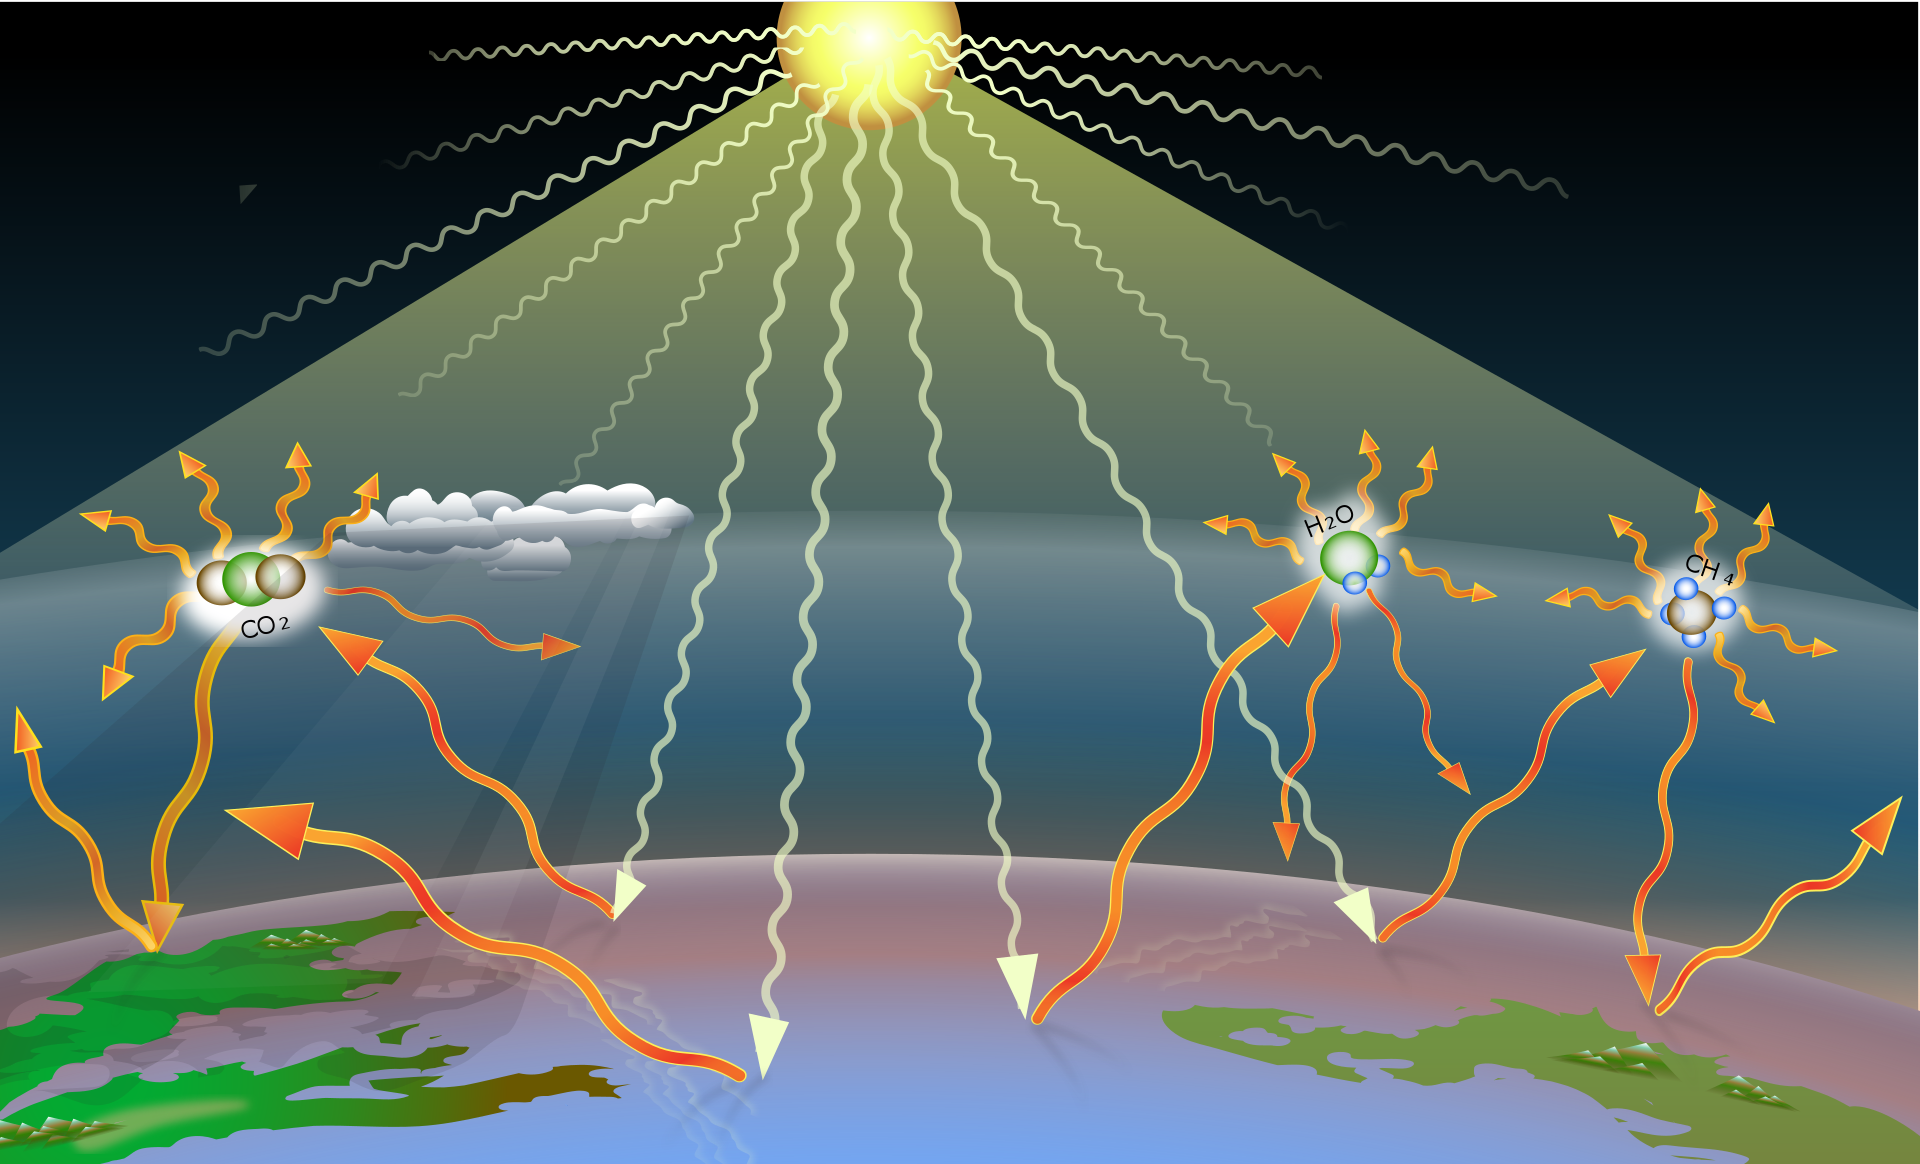
\includegraphics[width=1\textwidth]{Pic/Greenhouse-effect-t2.png}
\caption{The greenhouse effect: the radiation of the host star is captured by the planet and than remitted: this process is limited by the greenhouse molecules of the athomosphere that absorb and re-emit the radiation in all directions. Image taken from \cite{Greenhouse-effect-t2}}
\label{Greenhouse-effect-t2}
\end{center}
\end{figure}

\begin{figure}[h]
\begin{center}
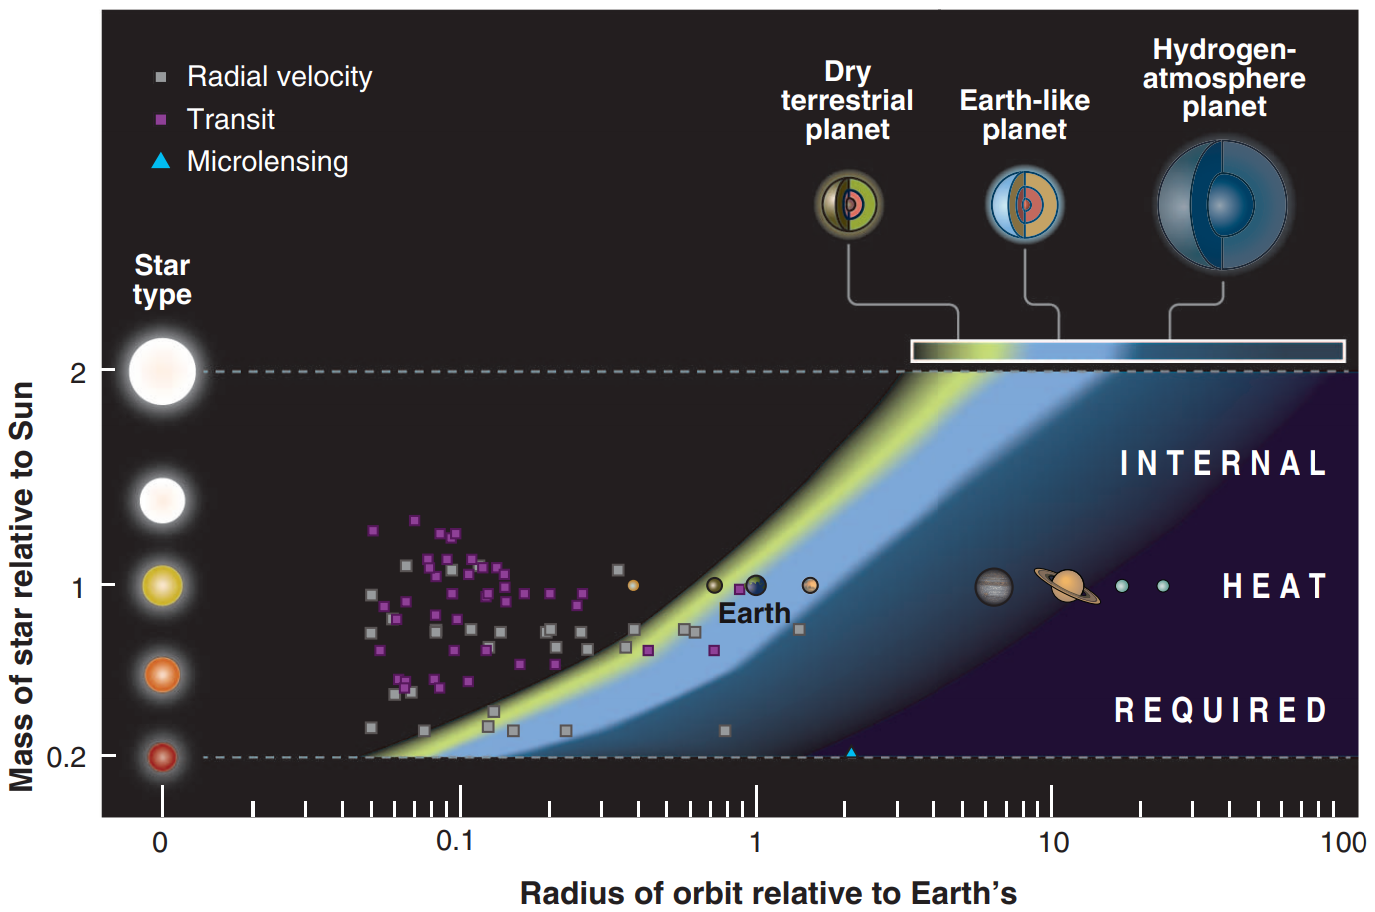
\includegraphics[width=1\textwidth]{Pic/Planets_habitability_Seager.png}
\caption{Seager representation of planet habitability as function of star type (that determinates the stellar activity) planet distance and its atmosphere: the light blue is the conventional habitable zone, while the dark blue and green one represent the extension of it due to the peculiarity of the planets. Image taken from \cite{seager2013exoplanet}}
\label{Planets_habitability_Seager}
\end{center}
\end{figure}


\clearpage

\section{Data Description}

The planet dataset was taken from the \textit{Planetary Habitability Laboratory @ UPR Arecibo} \cite{planet_dataset} website. Since the habitable planets, considering also the optimistic region, were  55 out of 3500, a reduction of the non-habitable planets to 445 was undertaken in order to make the habitable planets a significant portion of the overall set. As reported in table \ref{features_table}, among the different features that was provided by PHL, a restricted set was considered \footnote{The stellar spectral type named A,F,G,K,M and T (the methane dwarfs, their surface temperature spaces between 550-1300 K) were relabelled respectively as 1,2,3,4,5 and 6}: such operation was performed in order to avoid features whose causal effect on the habitability (where it was present) do not require very complex models/explanation. For all planets considered the features reported in the table \ref{features_table} were well-defined. 
 

\begin{table}[]
\caption{A selected features of the exoplanets dataset provided by PHL @ UPR Arecibo \cite{planet_dataset} accompanied by their measure unit }
\begin{tabular}{@{}lll@{}}
\toprule
Variable name                                                                & Abbreviation & Description/Comments                                                                                      \\ \midrule
Planet name                                                                  & P\_NAME      & \begin{tabular}[c]{@{}l@{}}The planet name according to \\ the international convention\end{tabular}      \\ \midrule
Planet Period                                                                & P\_P         & The planet period (days)                                                                                  \\ \midrule
Stellar temperature                                                          & S\_T         & \begin{tabular}[c]{@{}l@{}}The star effective temperature\\ (K)\end{tabular}                              \\ \midrule
Planet distance                                                              & P\_D         & \begin{tabular}[c]{@{}l@{}}Mean distance between the planet \\ and the host star (AU)\end{tabular}        \\ \midrule
Planet Periastron                                                            & P\_P         & \begin{tabular}[c]{@{}l@{}}The minimum distance between \\ the planet and the host star (AU)\end{tabular} \\ \midrule
Planet apastron                                                              & P\_A         & \begin{tabular}[c]{@{}l@{}}The maximum distance between \\ the planet and host star (AU)\end{tabular}     \\ \midrule
\begin{tabular}[c]{@{}l@{}}Planet effective \\ thermal distance\end{tabular} & P\_D\_E      & (AU)                                                                                                      \\ \midrule
\begin{tabular}[c]{@{}l@{}}Planet mean stellar\\ flux\end{tabular}           & P\_F         & (earth units)                                                                                             \\ \midrule
\begin{tabular}[c]{@{}l@{}}Planet equilibrium \\ temperature\end{tabular}    & P\_T\_E      & An albedo of 0.3 is considered (K)                                                                        \\ \midrule
Star radius estimated                                                        & S\_R\_E      & (solar units)                                                                                             \\ \midrule
Star luminosity                                                              & S\_L         & (solar units)                                                                                             \\ \midrule
Planet Habitability                                                          & P\_H         & 1 habitable, 0 else                                                                                       \\ \midrule
\begin{tabular}[c]{@{}l@{}}Estimated planet \\ radius\end{tabular}           & P\_R         & (earth units)                                                                                             \\ \midrule
\begin{tabular}[c]{@{}l@{}}Estimated planet\\ mass\end{tabular}              & P\_M         & (earth units)                                                                                             \\ \midrule
Star Spectral Type                                                           & S\_S\_T      & \begin{tabular}[c]{@{}l@{}}The star spectral type according\\ to the diagram in Fig. \ref{H_R_diagram} \end{tabular}         \\ \bottomrule
\end{tabular}
\label{features_table}
\end{table}

\begin{figure}[h]
\begin{center}
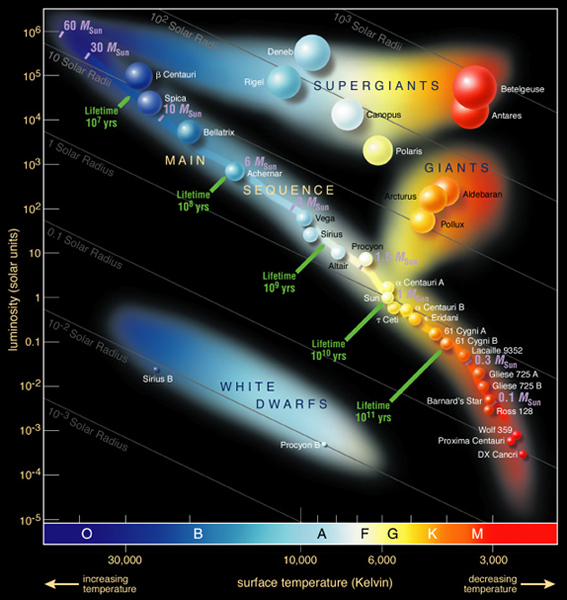
\includegraphics[width=0.9\textwidth]{Pic/S_T_T_explanation.png}
\caption{The Hertzsprung–Russell diagram (H-R): the phases that occurs during the lifetime of a star are placed on a plot that involves the surface temperature (and so the spectral type) vs the star luminosity .   Image taken from \cite{HR_diagram}}
\label{H_R_diagram}
\end{center}
\end{figure}


\clearpage

\section{Theoretical Background}

In this section the theoretical background of the methods used in this work are summarized following James at al. approach \cite{james2013introduction}. In particular here we considered the following ones: the decision tree, the random forest, the support vector classifier (for which a dimensionality reduction via the principal component analysis (PCA) was performed), the linear and the quadratic discriminant analysis. 
Before describing them, it is useful to recap the basic concepts that found the supervised learning.\newline\newline Lets consider a process, or more precisely a dynamical system,  where there is a set of variables \textbf{X} that represent the different initial conditions, called inputs, and a set of respective final condition, called outputs \textbf{Y}. Moreover lets suppose that the, during the first approach on the dynamical system the machinery of it is inaccessible (a black-box), but we are interested to predict some unknown output given some known input. Formally we are intended to approximate the dynamical system with the following relation \cite{james2013introduction}: 
\begin{equation}
\textbf{Y}=f(\textbf{X})+\epsilon
\end{equation}
where the $\epsilon$ represents the irreducible error term introduced by the approximation of the dynamical system (basically we will never know the exact laws that govern the phenomena, and also if these known we will always have an error term due to finite precision by which we approximate the initial conditions \cite{prigogine2018order,prigogine1997end,petrosky1996liouville}). Basically the aim of the statical learning theory is to estimate, with different methods, the response function $f$ \footnote{A useful approximation, especially in physics, of the response function is the linear response function $\chi(t-t')$ for an input h(t), where t represent the time, and an output x(t) is defined as $x(t)=\int_{-\infty}^{t}dt'\chi(t-t')h(t')+\epsilon$, where $\epsilon$ is due to the fact that we approximated the response function as a linear one. The linear response function is closely related to the Green function that plays a crucial role in the modern physics (for instance in the quantum field theory \cite{kubo1957statistical,zee2010quantum})}. It worth nothing that a very interesting application of this approach was performed by Claude Shannon \cite{shannon2001mathematical,mackay2003information} when he founded the information theory: in this case, as shown in Fig \ref{Noisy_channel} we can fix the input \textbf{X} as the signal produced and the output \textbf{Y} as the signal received, since no perfect channel is available the output signal will be distorted, thus the idea is how to infer from the output signal the input one.
\begin{figure}[h]
\begin{center}
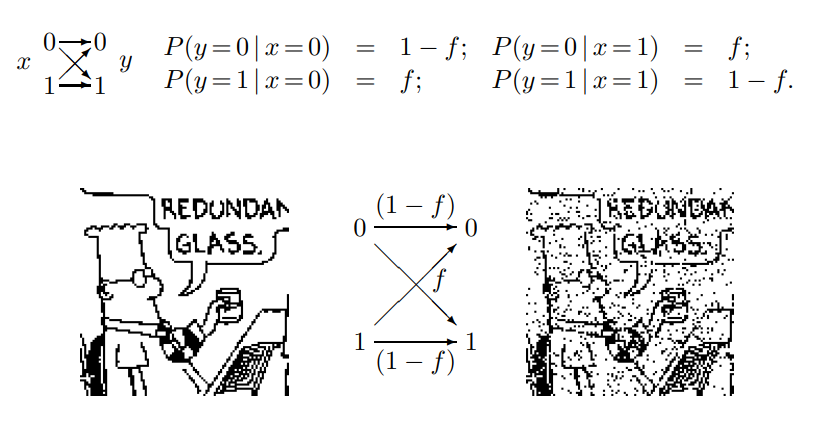
\includegraphics[width=0.9\textwidth]{Pic/Noisy_channel.png}
\caption{A sequence of binary data transmitted over a binary symmetric channel with noise equal to $f=0.1$   Image taken from \cite{mackay2003information}}
\label{Noisy_channel}
\end{center}
\end{figure}
Basically the approaches by which the problem of finding (inference) or forecasting (prediction) the behaviour of the response function is faced are two: the parametric methods and the non-parametric. The parametric methods perform firstly an approximation on the response function (e.g. it is linear), then use a part of the known input and output to estimate the parameters of the model by which the response function was approximated and finally the reaming values of input and output are used to validate the model; here the main risk is to introduce too much paramters that fits not only the response function but also the noise, thus when the input will be changed (with the test input/output) the error will abruptly increase: such behaviour is know as over-fitting. \footnote{The ovefitting can be quickly described with an Enrico Fermi answer to Freeman Dyson: "How many arbitrary parameters did you use for your calculations?" I thought for a moment about our cut-off procedures and said, "Four." He said, "I remember my friend Johnny von Neumann used to say, with four parameters I can fit an elephant, and with five I can make him wiggle his trunk." \cite{dyson}}. On the other side one can make no assumptions on the form of the response function (and so the model is more flexible) and try to estimate an f that is close as possible to the data point: these are the non-parametric methods; note that also in this case the over-fitting is possible. 


\clearpage

\subsection{Decision tree}

The basic idea of this approach is to divide the space of the predictor \textbf{X} in a set of a different subspaces, and then imposing that predictors that are in the same subspace have the same output value. Thus the problem is shifted to the creation of subspaces and their shape. Concerning the shape the most easy approach is to consider rectangles or, for higher dimensions, boxes; on the other side the creation of them can be performed by a top down approach where each box is divided in two sub-box, via the minimization of the RSS: given a predictor $X_{j}$ the cut-points s of boxes j are chosen so that, given \cite{james2013introduction}:   
\begin{equation}
R_{1}(j,s)= \{X | X_{j} < s \} \quad R_{2}(j,s)= \{X | X_{j} > s \}
\end{equation}
they minimize the following equation \cite{james2013introduction}: 
\begin{equation}
\sum_{i: x_{i} \in  R_{1}(j,s)}(y_{i}-\hat{y}_{R_{1}})^{2}+\sum_{i: x_{i} \in  R_{2}(j,s)}(y_{i}-\hat{y}_{R_{2}})^{2}
\end{equation}
where $\hat{y}_{R_{1}}$ represent the mean response for the training observation in $R_{1}(j,s)$. This splitting is performed recursively until each box contains no more than a fixed quantity of points. Finally the answer of the points contained in the same box will be identical. In order to avoid the overfitting one can consider to limit the splitting when the pay-off between the generation of a new subtree and the over-fitting threat is not convenient;formally this can be done by using the following expression \cite{james2013introduction}: 
\begin{equation}
\sum_{m=1}^{|T|}\sum_{x_{i}\in R_{m}}(y_{i}-\hat{y}_{R_{m}})^{2}+\alpha|T|
\end{equation}
where $\alpha$ represent the penalising factor when a new sub-tree is generated and |T| the number of terminal nodes of tree T. Such approach is called pruning. Finally if the output is class (as in this work: habitable or not) the RSS approach has to be replaced with the Gini index \footnote{This index was proposed by Corrado Gini to measure the inequality distribution of wealth in a country \cite{gini1912variabilita}}
\begin{equation}
G=\sum_{k=1}^{K}\hat{p}_{mk}(1-\hat{p}_{mk})
\end{equation}
or by the entropy \footnote{The entropy, introduced firstly by Rudolf Clausius and later developed by  Ludwig Boltzmann and Josiah Willard Gibbs, is concept that was initially introduced in physics: it was used to quantify the spontaneity of a transformation (\textgreek{entropía}-entropía, "a turning towards"). This because all the law of classical mechanics are symmetric with respect to the inversion of time and so the physical phenomena such as the diffusion of a gas (and not its spontaneous accumulation) cannot be explained only with them. Note that this issue, that was first formalized by \cite{loschmidt1876grosse,wu1975boltzmann}  was solved only recently with the fluctuation theorem \cite{evans1993probability,wang2002experimental}. The form used here is basically the scaled Gibbs expression (in which the Boltzmann constant $k_{b}$ was set to 1)}
\begin{equation}
D=-\sum_{k=1}^{K}\hat{p}_{mk}log\hat{p}_{mk}
\end{equation}
these indices, as evaluated here, measure the degree of purity of a node: if all the values are close to zero or one, their values will be close to 0. The decision tree approach provide therefore a results that is easily interpretable, drawable and communicable; on the other side among the statistical learning tools is not the one that provide the highest predictive accuracy and stability. 


\paragraph{Bagging}

In order to make the decision tree result more independent from the training dataset chosen (the over-fitting problem described before) one can consider to generate further training sets, via bootstrap method, in order to reduce the variance of the model. Thus the final model will be given by \\cite{james2013introduction}: 
\begin{equation}
\hat{f}_{bag}\left(x\right)=\dfrac{1}{B}\sum_{b=1}^{B}\hat{f}^{*b}\left(x\right)
\end{equation}
Where $B$ is the overall number of training sets generated via the bootstrap and $\hat{f}^{*b}$ the statistical model obtained from the $b^{th}$ training set. If a classification problem is undertaken, the class predicted will given by the one that is most common among the B predictions (majority rule).


\paragraph{Random forest} 
The random forest technique, firstly introduce in 1995 \cite{ho1995random}, represent an further improvement of the decision tree after the bagging: in this case, for each split, a random subset m of the full predictor set p is used. Such procedure is perform in order to avoid that the decision tree generated with the bootstrap are too similar due to the fact that there only few predictor that dominates the others, otherwise the reduction of variance due to the bagging is not so efficient since the bagged trees are correlated. The full random forest algorithm can be explained with the following analogy \cite{rand_for_exp}: lets consider a man, Carlo,  that would like to made a trip and, for this propose,  he asks to different people a suggestion; these asks to him a set of questions (last trip, sea or mountain, budget etc.) and give to him a final propose. Carlo at least takes a decision by using all the answers. In this example the different peoples are the bagged trees that give an answer basing of a different set of predictors. 
\begin{figure}[h]
\begin{center}
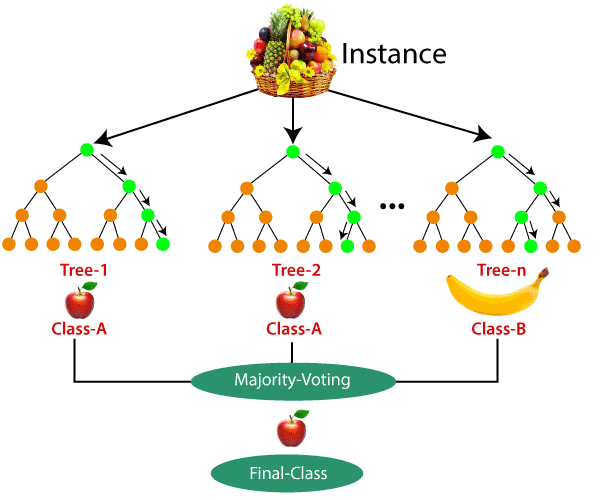
\includegraphics[width=0.9\textwidth]{Pic/random-forest-algorithm2.png}
\caption{A schematic representation of the random forest algorithm. Image taken from \cite{rand_for_fig}}
\label{Noisy_channel}
\end{center}
\end{figure}

\clearpage
\section{Results and discussion}

\clearpage

\section{Conclusions}

\clearpage

\section{R code}
\begin{lstlisting}


\end{lstlisting}
%------------------------------------------------



%----------------------------------------------------------------------------------------
%	BIBLIOGRAPHY
%----------------------------------------------------------------------------------------

\renewcommand{\refname}{\spacedlowsmallcaps{References}} % For modifying the bibliography heading

\bibliographystyle{unsrt}

\bibliography{bibliography.bib} % The file containing the bibliography

%----------------------------------------------------------------------------------------

\end{document}